\section{Introduction}

In their paper, \citet{dowd2011estimating} propose a model to gain a deeper understanding of the behavior of seals (Callorhinus ursinus) in their natural habitat, using data on their vertical velocity. The researchers placed sensors on the seals, which enabled them to track the seals' depth at regular intervals. The intention is to use this measure as a proxy for inferring the seals' behavior. Specifically, the depth measurements vary depending on whether the seals are hunting, exploring, moving, and so on. To do so, they model the animal's behavior with state-space models using high resolution time series data. Doing so, they introduce latent behavioral parameters, that reflect the comportment of the seals. This approach can then be applicable to most horizontal and vertical movement models using high-resolution tag data.

% The objective of this study is to gain a deeper understanding of the behavior of seals (Callorhinus ursinus) using data on their vertical velocity. The researchers placed sensors on the seals, which enabled them to track the seals' depth at regular intervals. The intention is to use this measure as a proxy for inferring the seals' behavior. Specifically, the depth measurements vary depending on whether the seals are hunting, exploring, moving, and so on.

\section{Formalism and first equations}

% To address this problem, we consider the following stochastic movement model:
To address this problem, we want to construct a stochastic animal movement model using a state-space model.
The first part of the model is the state evolution equation :
\begin{equation}
\mathbf{x}_t=\mathbf{f}(\mathbf{x}_{t-1},\mathbf{\theta}_t)+\mathbf{n}_t
\end{equation}
where $\mathbf{x}_t$ represents the vertical velocity, $\theta_t$ the latent behavioral parameters, $\mathbf{f}$ characterizes the movement and $\mathbf{n}_t$ is the system noise. However, it is not ideal to use such a state-space model in this context, because we would prefer the sought-after value $\theta_t$ to follow a Markov process, rather than the observed value $\mathbf{x}_t$.
To overcome this issue, we artificially augment the state space by introducing the variable $X_t = \begin{pmatrix}
\mathbf{x}_t\\\theta_t
\end{pmatrix}$.

The second part, is the observation equation given by $y_t = HX_t + e_t$, where $H = (1, 0)$, so that $y_t$ represents the observation of vertical velocity at time $t$, and $e_t$, the observation error, is a normal noise term.

We seek a Markov process of the form:
\begin{equation}
\begin{pmatrix}
\mathbf{x}_t\\\theta_t
\end{pmatrix}
=
\mathbf{f}\begin{pmatrix}
\mathbf{x}_{t-1}\\\theta_{t-1}
\end{pmatrix}
+
\begin{pmatrix}
\mathbf{n}_t \\\mathbf{v}_t
\end{pmatrix}
\end{equation}

Unfortunately, there is no consistent model for representing the evolution of $\theta_t$. The solution proposed by the authors is as follows: although there is no model for $\theta_t$ over a long period, it is consistent to say that this parameter is constant over short periods. Recall that this parameter models the behavior (hunting, exploring, moving...) of the seal. It is therefore assumed that over a period of 26 minutes (see details in the appendix), the behavior, and therefore the parameter, is constant.

We therefore consider a window of 26 minutes, under the assumption that $\theta_t$ is constant. Even in this simplified case, a particle filter does not allow us to estimate the value of $\theta_t$ since it would be fixed. The authors therefore introduced an arbitrary movement on $\theta_t$ in order to be able to estimate it. We would therefore have:
$$
\theta_t = \theta_{t-1} + v_t
$$
where $v_t$ follows a normal distribution with variance $\sigma_v^2$.\\


However, by introducing this arbitrary movement of $\theta_t$, we also increase the variance in its estimation, especially if $\sigma_v^2$ is large. We therefore want a small value of $\sigma_v^2$. However, if it is too small, we find ourselves in the limiting case where the parameter value is constant and cannot reach its "true value".
We will therefore proceed iteratively, gradually reducing the value of $\sigma_v^2$.\\

\begin{algorithm}
\caption{Estimation of $\theta$ on the i-th window $w_i = [y_1, \dots ,y_T]$}
\label{alg:Estimation}
\begin{algorithmic}[1]
% \Require A time window $w_i = [y_1, \dots ,y_T]$
% \Ensure An estimation of $\theta_i$ on the window
\State $m \gets 0$ \Comment{The iteration step}
\State $\sigma_v^2(0) \gets 0.1$ \Comment{The parameter noise variance}
\State $\theta_0(0) \gets 0$ \Comment{The initial value of the parameter}
\While{$m < 10$}
\State Estimate $\theta_{1,\dots,T}(m)$ using a particle filter and initial values $\theta_0(m)$ and $\sigma_v^2(m)$
\State Update $\theta_0(m+1) \gets \frac{1}{T}\sum_{t = 1}^{T}\theta_t^m$
\State Update $\sigma_v^2(m+1) \gets \alpha\times\sigma_v^2(m)$ \Comment{We reduce the variance to narrow on the value of $\theta_i$}
\EndWhile
\State Use $\theta_0(10)$ as the estimation for $\theta_i$
\end{algorithmic}
\end{algorithm}

This time, we have a consistent estimation of $\theta$ for each time window. From them, we can reconstruct the latent behavior parameters and its evolution in time.

\section{Definition of the movement model}
To complete the implementation of the algorithm, we need to define $\mathbf{f}$, which characterizes the movement of the seal. The authors have chosen the following $AR(2)$ model to describe the evolution of velocity on a single axis:
\begin{equation}
z_t = a_1z_{t-1} + a_2z_{t-2} + \epsilon_t
\end{equation}
This equation is not in the form of a Markov process, which is what we desire:
$$
z_t = \mathbf{f}(z_{t-1}, \theta_t) + \epsilon_t
$$
where $\theta_t = \begin{pmatrix}
    a_{1,t}\\ a_{2,t}
\end{pmatrix}$.\\

To remedy this, the authors have augmented the state space with the dummy variable $\zeta_t$, such that:
\begin{equation}
\begin{pmatrix}
\mathbf{z}_t\\\mathbf{\zeta}_t
\end{pmatrix}
=
\begin{pmatrix}
a_{1,t}& a_{2,t} \\
1 & 0
\end{pmatrix}
\begin{pmatrix}
\mathbf{z}_{t-1}\\\mathbf{\zeta}_{t-1}
\end{pmatrix}
+
\begin{pmatrix}
\mathbf{\epsilon}_t \\ 0
\end{pmatrix}
\end{equation}
This allows us to obtain a Markov process, which can then be filtered using a particle filter.

\section{Final form}
Taking into account both state augmentations, we end up with the movement model :
\begin{equation}
\label{eqn:markov process}
    \mathbf{X_t} =
    \begin{pmatrix}
    \mathbf{z_t}\\\mathbf{\zeta_t}\\ a_{1,t}\\ a_{2,t}
    \end{pmatrix}
    =
    \begin{pmatrix}
    a_{1,t-1}& a_{2,t-1} & 0 & 0\\
    1 & 0 & 0 & 0\\
    0 & 0 & 1 & 0\\
    0 & 0 & 0 & 1\\

    \end{pmatrix}
    \begin{pmatrix}
    \mathbf{z}_{t-1}\\\mathbf{\zeta}_{t-1}\\ a_{1, t-1} \\ a_{2,t-1}
    \end{pmatrix}
    +
    \begin{pmatrix}
    \mathbf{\varepsilon}_t \\ 0 \\ \nu_{1,t} \\\nu_{2,t}
    \end{pmatrix}
\end{equation}
with $z_t$ the vertical velocity, $\zeta_t = z_{t-1}$ a dummy variable and $(a_{1, t-1}, a_{2,t-1})$ representing the latent behavior parameters. The system noise $\varepsilon_t$ takes the form of a normal mixture process that allows for occasional large values, $\varepsilon_t \sim 0.9 \Norm{0}{\sigma_{\varepsilon}^2} + 0.1 \Norm{0}{10\sigma_{\varepsilon}^2}$. Meanwhile, $\nu_{1,t}$ and $\nu_{2,t}$ are random noise for the random walk of the parameters, $\nu_{1,t}, \nu_{2,t} \sim \Norm{0}{\sigma_{\nu}^2}$. The equation can be rewritten as \mbox{$\mathbf{X}_t = M_t \mathbf{X}_{t-1} + \mathbf{\hat{n}_t}$}.

And the observation model :
\begin{equation}
\label{eqn:y sachant X}
    \mathbf{y}_t =
    \begin{pmatrix}
    1 & 0 & 0 & 0
    \end{pmatrix}
    \begin{pmatrix}
        \mathbf{z_t}\\\mathbf{\zeta_t}\\a_{1,t}\\ a_{2,t}
    \end{pmatrix}
    +
    \mathbf{e_t}
\end{equation}
with the observation error $\mathbf{e_t} \sim \Norm{0}{\sigma_{o}^2}$. It can be rewritten as $\mathbf{y}_t = G_t \mathbf{X_t} + \mathbf{e_t}$.

The system noise and observation error variance are estimated beforehand on each window, using the method proposed in the paper that relies on a quadratic regression of the ACVF.

This leads to the associated Feynman-Kac model where :
\begin{itemize}
    \item $M_t$ is the Hidden Markov Process described in (Eq. \ref{eqn:markov process}).
    \item $G_t$ is the density of $\mathbf{y_t}$ knowing $\mathbf{X_t}$ (Eq. \ref{eqn:y sachant X}).
\end{itemize}

\section{Construction of the windows}
We now have an algorithm that allows us to estimate $a_1, a_2$ over a time minute window. We remind you that on this window, these parameters are estimated to be constant. In order to minimize the error induced by this assumption, the authors choose to overlap windows in order to have a better estimation of $a_1, a_2$ over a longer period. More specifically, they use a 26 minute sliding window that moves 13 minutes at a time. This way, for each time $t$, they have two estimations of $a_1, a_2$ so that it is possible to take the mean and hence soften the possible huge gap between values.


\section{Simulation and results}
In this section, we will present the results we obtained ourselves, on real data, we choose to use our results on the day 18/01/2008. To run the simulation, we used the Python \texttt{particles} package. The code is available on GitHub \url{https://github.com/gwatkinson/smc_movement_models}. A small package was made to organize the functions, and the simulations were run in the two main notebooks.

\subsection{Simulations}
The \textsc{Figure} \ref{fig:data} presents the data used in our experiment. The first subfigure presents the evolution of the depth of the seal on January 18th, 2008. Whereas the second presents the vertical velocity, which is used in our state space model.

We notice three different behavioral periods:
\begin{enumerate}
    \item From 00:00 to 6:00, we have a series of occasional deep dives, that can be interpreted as explorations.
    \item From 6:00 to 12:00, the vertical speed is quite constant, this could correspond to a period of rest or to a period of travel.
    \item From 15:00 to 21:00, we have a quick series of shorter dive, that correspond to the behavior of a seal hunting.
\end{enumerate}

We thus want latent parameters estimate, that translates those states in a mathematical representation easier to analyze at scale.

\begin{figure}
\centering
    \begin{subfigure}[t]{0.45\linewidth}
        \centering
        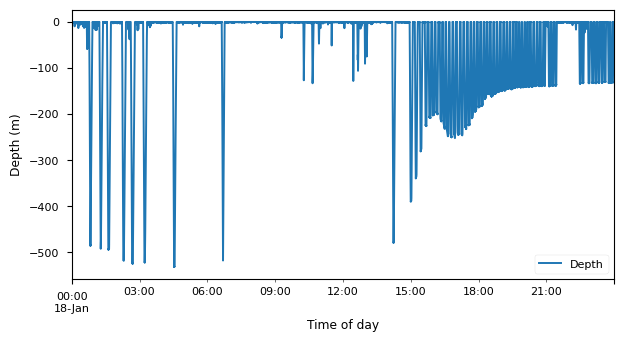
\includegraphics[width=\linewidth]{images/depth_fig.png}
        \caption{Evolution of the depth (in m) of the seal on January 18th, 2008, taken at 5 second intervals.}
        \label{fig:depth}
    \end{subfigure}
    \begin{subfigure}[t]{0.45\linewidth}
        \centering
        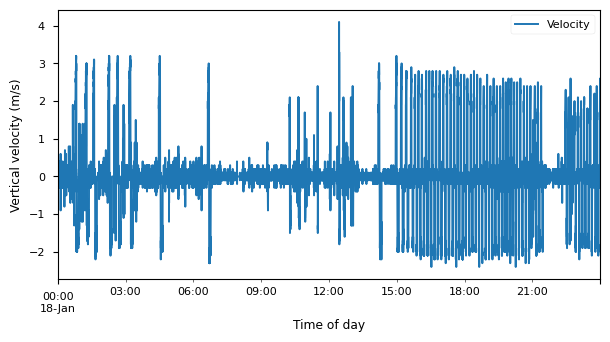
\includegraphics[width=\linewidth]{images/velocity_fig.png}
        \caption{Evolution of the vertical velocity (in m/s).}
        \label{fig:velocity}
    \end{subfigure}
\caption{Data of the depth and vertical velocity of a single seal on January 18th, 2008.}
\label{fig:data}
\end{figure}

\subsection{Results using the algorithm from the paper}
The \textsc{Figure} \ref{fig:parameter estimation} shows the results obtained on that day using the algorithm \ref{alg:Estimation}, for parameters $a_1, a_2$. We ran the algorithm 20 times, to estimate the variance of the parameters in each window.  As expected, we have quite stable value for one chosen behavior. Furthermore, the three different behavioral periods evoked above are well represented. At first, we see short spikes corresponding to the exploration. In the middle, the values of $a_1$ and $a_2$ are minimal. Then, during the hinting phase, $a_1$ is close to $0.8$, while $a_2$ is close to $0.3$. The phases are clearly separated.

\begin{figure}
\centering
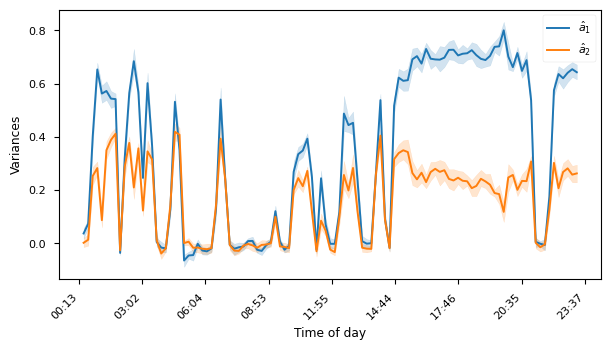
\includegraphics[width=0.8\linewidth]{images/a1_a2_var_0.5.png}
\caption{Results of the algorithm to estimate $a_1$ and $a_2$. We ran the algorithm 20 times to estimate the variance of the parameters on each time window.}
\label{fig:parameter estimation}
\end{figure}

\section{How to use SMC$^2$ within this context}
In that section, we do not assume anymore that $a_1, a_2$ follows a random walk on each window. They are now supposed constant.
This allows us to avoid the augmented state and the Markov process used to define the Feynman-Kac model becomes the following:
\begin{equation}
    \mathbf{X_t} =
    \begin{pmatrix}
    \mathbf{z_t}\\\mathbf{\zeta_t}
    \end{pmatrix}
    =
    \begin{pmatrix}
    a_1& a_2\\
    1 & 0

    \end{pmatrix}
    \begin{pmatrix}
    \mathbf{z}_{t-1}\\\mathbf{\zeta}_{t-1}
    \end{pmatrix}
    +
    \begin{pmatrix}
    \mathbf{\epsilon}_t \\ 0
    \end{pmatrix}
\end{equation}

An SMC defined with this Hidden Markov Process will return an estimation of for all $t, \mathbb{P}^{a_1,a_2}(y_{0:T})$.
To be able to have a good approximation of  of the latent parameters $a_1, a_2$, we would like to estimate the density function:
$$
(a_1, a_2) \xrightarrow{} \mathbb{P}^{a_1,a_2}(y_{0:T})
$$

 It is possible to do that with a SMC sampler.
 Following the formalism in the algorithm of an SMC sampler given in \cite{dowd2011estimating} in section 17, algorithm 17.1, $\gamma_i(a_1, a_2) = \mathbb{P}^{a_1,a_2}(y_{0:T})$ would be computed using the particle filter described by the Hidden Markov Process above.
 $M_i$ is just a random walk and allows to go from $(a_1^{i-1}, a_2^{i+1})$ to $(a_1^i, a_2^i)$.

 The \textsc{Figure} \ref{fig:SMC2} present the results using the SMC$^2$ sampler. Compared to the previous algorithm, we distinguish the same trends. However, the values of the parameters are quite different, especially during the hunting phase, where $a_1$ is a lot smaller ($0.5$ compared to $0.8$).

 \begin{figure}
\centering
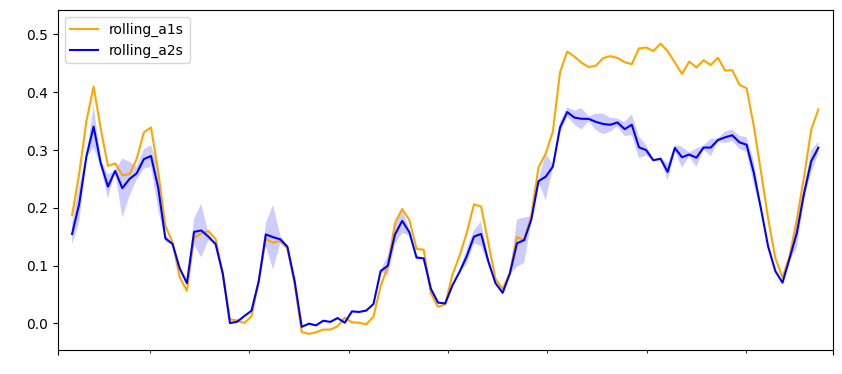
\includegraphics[width=0.8\linewidth]{images/results_with_uncertainty_SMC2_cropped.png}
\caption{Results of the SMC$^2$ to estimate $a_1, a_2$.}
\label{fig:SMC2}
\end{figure}

% \clearpage
\section{Conclusion}
The main purpose of this paper is to propose an augmented state-space model to estimate the behavioral parameters of seals in Alaska, USA.
Such a model can be used to estimate latent parameters, describing the behavior of the animals.

The authors made several assumptions to obtain meaningful results. First, instead of estimating the value of the behavioral parameter per unit of time (every five seconds), they created \textit{time window} in order to obtain smooth varying parameters in time (between each time window). For this purpose, particle filters were applied on each time window in order to estimate the behavioral parameter $\theta = (a_1, a_2)$, where $a_1$ and $a_2$ are the coefficients of the AR(2) series of the vertical velocity: $z_t = a_1z_{t-1} + a_2z_{t_2} + \varepsilon_t$. One of the first important assumptions made by the authors, is to model $(a_1, a_2)$  as a random walk on each time window. This allows us to apply an SMC filter to estimate these parameters more easily. Then, in order to distinguish the errors due to the observations and the systemic errors due to the movement of the model, the authors assume that the former are uncorrelated in time. This allows to estimate more easily $\sigma_\varepsilon^2$ and $\sigma_z^2$ "offline", before applying the SMC.

The interest here is to apply a SMC$^2$ filter in order to get rid of the hypothesis of variation of $a_1$ and $a_2$ in a time window. The results are in this case more precise since they have a smaller variance. It enables to make less assumptions and gives another perspective on the data.
